\chapter{Introduction}
\label{cha:intro}
\epigraph{The best weapon of a dictatorship is secrecy, but the best weapon of a democracy should be the weapon of openness.} 
{\textit{Niels Bohr}} 

\section{Problem Statement}
A democracy can be best described as a system where all eligible voters have equal rights to express their opinion(s) on different matters. 
One of the most important example of expressing opinion is by holding election to elect the leader of country. During the 
election, all eligible voters express their opinion on a paper,  known as ballot,  in a manner, depending on the voting method, 
which reflects their true intention.  For example, if the voting method is \textit{ranked voting (preferential voting)},  the voters rank the 
candidates according to their preference, and if the method is \textit{first past the post},  each voter selects one candidate by marking
against the candidate name on the ballot. Later, once the ballot cast finishes, a candidate is elected as a winner from  the participating
candidates by combing the choices of all the voters. 
The paper ballot method works great, except it is very time consuming, expensive, error prone, 
and not very inclusive for disabled voters such as the visually impaired.
In order to solve the various problems posed by paper ballot, many countries are adopting electronic voting as an alternative. 
Electronic voting is 
getting popular in many countries, and the reason for its popularity is cost-effective, faster result, high voter turn out, 
and accessible for disabled voters.  
Undeniably, electronic voting has helped, for example, Australia to ease the logistic challenges of elections because of its massive land size and sparse
population and save millions of dollars.  In addition, it has helped India, the second most populous country with 900 million eligible voter, to declare 
2019 election with 67 percent voter turn out (roughly 600 million) in 2 days, and  Estonia, a labour shortage country, has saved 
thousands of man hours, 11,000 working days, by using electronic voting \citep{Estonia}.

   
  Despite all these benefits, electronic voting is an arduous effort because a minuscule possibility of 
  going anything wrong in software or hardware could lead to an undesirable situation \citep{TSwiss},
  \citep{10.1007/978-3-319-22270-7_3}, \citep{ARANHA2019335},
  \citep{Feldman:2007:SAD:1323111.1323113}.  The nature of (electronic) data and the ease of 
  its manipulability/misinterpretation causes electronic voting many problems, which are not present in paper ballot elections, that 
  makes it perfectly susceptible to delivering wrong and unverifiable results \citep{Wolchok:2010:SAI:1866307.1866309}.
  For instance,  if a software program used in electronic voting 
  for reading the ballots has byte order bug, or even if it depends on some other software which has byte order bug (the data is supposed to read 
  from left to right, but software is reading right to left), then the interpretation of 
  a ballot would be completely different from what the voter had in mind.
  More often than not, these software programs are configured incorrectly \citep{1301313} and run at the top of (untrusted) operating 
  systems and hardware. Usually, operating systems have millions of lines of code (for example, Linux has 15 millions lines) which exposes
  a large attack surface and could be exploited, possibly by the current government or foreign countries, for illegal gain.
  The worst, these software and hardware  are commercial in 
  confidence and treated as a black-box, and, most often, their source code or design is not open 
  for public scrutiny \citep{AEC:2013:LMM}. In addition, these software programs 
  take a list of ballots and produce the result without producing any evidence about the correctness of result.  As a consequence,
  from casting the ballot electronically to declaring winner based on the cast (electronic) ballot, the whole process lacks basic assumptions
  of democracy such as transparency, genuineness, and verifiability. 
  
  In order to make the electronic voting process genuine and trustworthy, the electronic voting 
  research community has recognised some must-have properties of electronic voting protocol
  \citep{5958051}, 
   \citep{Benaloh:1994:RSE:195058.195407},  \citep{Delaune:2010:VPT}, \citep{Bernhard:2017:PES}:
  

 \begin{itemize}
 
  \item Correctness:
 	The produced results are correct and convincing to all leaving no  ground for suspicion. 

 \item Coercion-resistance: A voter can not cooperate with a coercer to prove anything about her choices.
 
 \item Eligibility: Only eligible voters can cast a ballot.
 	
 \item Privacy:
    All the votes must be secret, and a voter should not be able to convince anyone the 
    value of her vote.
 
 \item End-to-end Verifiability:
 Any independent third party should be able to verify the final outcome of election based on cast 
 ballots.  It can be further divided into three sub-categories:
 
 \begin{itemize}
  \item Cast-as-intended: Every voter can verify that their ballot was cast as
  intended.
  \item Collected-as-cast: Every voter can verify that their ballot was collected as
  cast.
  \item Tallied-as-cast: Everyone can verify the final result on the basis of the
  collected ballots.
\end{itemize}
\end{itemize}
	

In this thesis, we focus on privacy, correctness, coercion-resistance, and tallied-as-cast, the third part of end-to-end verifiability, property 
of an election. Furthermore, we assume that the first two properties of end-to-end verifiability, cast-as-intended and 
collected-as-cast, hold for an election. Cast-as-intended is a verification method that is used to audit the 
front end voting software, 
also known as voting client software, to make sure that it is not modifying the options of voters. In a nutshell, 
the cast-as-intended is assurance to a voter that front-end software is transparent and her vote 
is recorded according to her intent.  Cast-as-intended is an active area of research in its own right \citep{10.1007/978-3-319-22270-7_1},  \citep{mci/Marky2018},  \citep{cortier:hal-02346420}; 
however, it is not the focus of this thesis. Similarly,  collect-as-cast is a notion related to the voters to make 
sure that the ballots appearing on the bulletin board are indeed the ballots that cast during the election. A consequence 
of collected-as-cast notion is that any attempt to change or delete the ballots from the bulletin board would 
be detected. This notion is indeed a crucial one and works as a bridge between the cast-as-intended and tallied-as-cast 
notions. However, it is related to voters' behaviour; hence, the reason for assumption.  Moreover, assuming these two 
notions, cast-as-intended and collected-as-cast, helped us in isolating the irrelevant details and 
paved a way to focus more on the complex problem of counting, i.e. tallied-as-cast. 


\section{Research Motivation and Contribution}
Given the potential advantages of electronic voting,  we need to address
the correctness, privacy, and verifiability concerns for its widespread adoption. 
This thesis sets out to address these concerns of electronic voting. 
The questions we asked ourselves were:
 \begin{enumerate} 
  \item Can we implement a vote counting protocol with a "guarantee"
  (maximum possible assurance that we can get about software programs
   with respect to some specification) 
   that the resulting implementation is correct and  practical enough
    to count  millions of ballots in a real-life election (Correctness)?

  \item Can we produce the result by counting encrypted ballots without revealing 
  its content, and at the same time, 
  assuring everyone that the result produced is only based on "valid" ballots, 
  and "invalid" ones have been discarded  (Privacy and Coercion-resistance)?
 \item Can we decouple the verifiability from the implementation details of a vote counting software program, i.e. 
    generating enough evidence so that any independent auditor can 
    ascertain the outcome of an election without trusting the implementation 
    of the vote counting software program used to conduct the election (Verifiability)?
  \end{enumerate}


In order to answer these questions, at first we need two things: (i) a voting protocol and 
(ii) a tool to implement the voting protocol and prove the correctness properties of the implementation. 
Our choice of voting protocol is the   Schulze method \citep{Schulze:2011:NMC} and 
the tool is Coq \citep{Bertot:2004:ITP} theorem prover  for implementing and proving 
the correctness of  the Schulze method.
Even though the Schulze method is not used in any democratic election to public office,
it is one of the most popular method to elect candidates for various organisations, e.g. Debian, GnuPG, 
KDE,  etc., over the Internet and political groups,  e.g.  pirate party of Australia, Belgium, Brazil, 
Germany, etc\footnote{\url{https://en.wikipedia.org/wiki/Schulze_method#Users}}.
One of the major reason for its popularity is that it has many desirable properties.
While no preferential voting scheme can guarantee all desirable properties that one would
like to impose due to Arrow’s theorem \citep{Arrow:1950:DCS}, the Schulze method offers a good compromise, 
with a number of important properties already  established  in  Schulze’s  original  paper. 
Amongst the various  properties, the Schulze method satisfies the \textit{resolvability criterion}, 
i.e. it elects a single winner under the assumption that number of voters are much larger than
 number of candidates (and in case of a tie, when there is more than one winner, a random vote can be 
selected to declare the winner.  However, our formalisation 
has not taken the randomness into account, so it can produce more than one winner). 


Coq is a theorem prover (proof assistant) based on the \textit{Calculus of Inductive Construction (CIC)} 
\citep{Coquand:1988:CC:47724.47725} \citep{coquand1988inductively}. 
The calculus of inductive construction is a highly expressive formal system (type system) 
which allows "proof" terms and 
"computation" terms to live in the same universe (level). Moreover, during the proof development, 
it provides step by step feedback to the user and the possibility to automate proofs by 
writing custom tactics using the Ltac \citep{10.5555/1765236.1765246}. In addition, 
Coq proofs can be extracted into the  Haskell, OCaml, and Scheme.
 
Now that we have the voting protocol (Schulze method) and  the tool (Coq theorem prover), 
we demonstrate that it is possible to achieve correctness, privacy, coercion-resistance, and (tallied-as-cast) verifiability in 
electronic voting. We achieve the following:
\begin{itemize}
 \item \textit{Correctness} by formally specifying the Schulze method  and prove its correctness properties
  inside the Coq theorem prover. 
 Coq has a well-developed extraction facility that 
 we use to extract proofs into OCaml programs, and using these extracted OCaml programs, we 
 have counted the ballots from an election to produce the result. 
 \item \textit{Privacy and Coercion-resistance} by encryption. We use homomorphic encryption to compute the 
  final tally without decrypting any individual ballot.  The encryption hides the preference of voters, facilitating 
  ballot privacy and preventing any possible coercion.  
  
\item \textit{Verifiability} by tabulating the relevant data of an election (which we call the scrutiny-sheet/certificate).
   Achieving verifiability in a plaintext ballot counting is fairly straightforward. 
   To achieve verifiability in encrypted ballot counting, 
   we augment the scrutiny sheet with zero-knowledge proofs for each claim we make during the 
   counting, which can  later be checked by any auditor.  
\end{itemize}



In addition to demonstrating correctness, privacy, and verifiability, we have also developed a formally verified certificate 
checker. Moreover, we have shown that our implementation adheres to the various properties established by Schulze in 
his original paper. 

\noindent 
\textit{Formally Verified Checker:} Third party independent election audit based on scrutiny sheet data is a crucial step towards 
establishing the trust in the system.   However, auditing the scrutiny sheet of an election involving encrypted ballots
is not straightforward in comparison to an election with plaintext ballots. 
In general, auditing the scrutiny sheet of an election involving 
plaintext ballots simply requires the knowledge of basic arithmetic, e.g.~addition, subtraction and multiplication, 
and virtually anyone can audit the election based on the data produced in the scrutiny sheet by
using a calculator or by writing a simple program in her preferred language. 
However, an encrypted ballot election scrutiny sheet involves various
cryptographic concepts (homomorphic encryption, zero-knowledge proof, commitment scheme, etc.) 
which are accessible to very few voters, mainly cryptographers,  so auditing it 
requires a deep understanding of cryptographic principals. To ease this situation, we have developed a formally verified 
certificate checker as a proof of concept for automating the audit of an election, conducted on encrypted ballots. 
Having said that,  our certificate generated by encrypted ballots is very complex, and formalizing all the cryptographic 
primitives involved would be fairly time consuming, so we have developed a proof of concept 
formally verified certificate checker for the International Association of Cryptologic Research (IACR) 2018 election
scrutiny sheet (the IACR scrutiny sheet is relatively simple compared to our certificate).

\noindent
\textit{Properties of Schulze Method:} We have proved two properties,  Condercet winner and Reversal symmetry 
amongst many, of the Schulze method inside the Coq theorem prover (ongoing work).  These properties could be seen as an 
ultimate stress testing for an implementation, and we have shown that our implementation of the Schulze 
method follows two important properties,  i.e.  Condercet winner and Reversal symmetry.  Ideally,  
we would like to prove that our implementation follows all the properties established in the Schulze's 
paper  \citep{Schulze:2011:NMC}.


\section{Cryptographic Blackbox}
Since the beginning of this project, our primary goal was 
to achieve privacy (using encryption) and verifiability (using zero-knowledge proof) in electronic voting 
using cryptographic primitives (but not the verification of primitives itself). 
To achieve this goal, we have 
taken the axiomatic approach and assumed the existence of cryptographic primitives 
inside Coq. Moreover, we assume axioms about their correctness behaviour, e.g.~decryption 
is left inverse of encryption. These primitives, in general, provide functionality 
of generating a random permutation, encrypting a plaintext data, decrypting a ciphertext data, 
producing commitment of a value, constructing a zero-knowledge proof, 
and verifying a zero-knowledge proof. Later, in extracted OCaml code from Coq code, these functions are instantiated 
with Unicrypt \citep{LocherH14} functions\footnote{Formalising the whole cryptographic stack used in our 
project would be very time consuming (probably a PhD itself), but it would be worth trying. 
Although, we have formalised the (ElGamal) encryption, and decryption inside Coq, but we still 
are very far from achieving the goal of fully verified cryptographic stack.  We leave the formalisation 
of cryptographic primitives for future work (work in progress).}.



\section{Publication}
 The chapters, or some part of it,  of this thesis are based on the following papers:
	\begin{enumerate}
	\item Pattinson D., Tiwari M. (2017) Schulze Voting as Evidence Carrying Computation. In: Ayala-Rincón M., Muñoz C. 
	(eds) Interactive Theorem Proving. ITP 2017. Lecture Notes in Computer Science, vol 10499. Springer, Cham.  \url{https://doi.org/10.1007/978-3-319-66107-0_26}
	\item Bennett Moses L., Goré R., Levy R., Pattinson D., Tiwari M. (2017) No More Excuses: Automated Synthesis of Practical and Verifiable Vote-Counting 
	Programs for Complex Voting Schemes. In: Krimmer R., Volkamer M., Braun Binder N., Kersting N., Pereira O., Schürmann C. (eds) Electronic Voting. E-Vote-ID 
	2017. Lecture Notes in Computer Science, vol 10615. Springer, Cham. \url{https://doi.org/10.1007/978-3-319-68687-5_5}
	\item Ghale M.K., Goré R., Pattinson D., Tiwari M. (2018) Modular Formalisation and Verification of STV Algorithms. In: Krimmer R. et al. (eds) Electronic 
	Voting. E-Vote-ID 2018. Lecture Notes in Computer Science, vol 11143. Springer, Cham.  \url{https://doi.org/10.1007/978-3-030-00419-4_4}
	\item Haines T., Pattinson D., Tiwari M. (2020) Verifiable Homomorphic Tallying for the Schulze Vote Counting Scheme. In: Chakraborty S., Navas J. (eds) 
	Verified Software. Theories, Tools, and Experiments. VSTTE 2019. Lecture Notes in Computer Science, vol 12031. Springer, Cham. \url{https://doi.org/10.1007/978-3-030-41600-3_4}
	\item Thomas Haines, Rajeev Goré, and Mukesh Tiwari. 2019. Verified Verifiers for Verifying Elections. In Proceedings of the 2019 ACM SIGSAC Conference on 
	Computer and Communications Security (CCS '19). Association for Computing Machinery, New York, NY, USA, 685–702. DOI:\url{https://doi.org/10.1145/3319535.3354247}
	\end{enumerate}
 \noindent
 Part of chapter \ref{cha:background} is based on \textit{No More Excuses: Automated Synthesis of Practical 
 and Verifiable Vote-Counting Programs for Complex Voting  Schemes},
 chapter \ref{cha:schulze_method} is based on \textit{Schulze Voting as Evidence Carrying Computation},
 chapter \ref{cha:homormorphic_schulze} is based on \textit{Verifiable Homomorphic Tallying for the 
 Schulze Vote Counting Scheme}, and part of chapter
 \ref{cha:software_independence} is based on \textit{Verified Verifiers for Verifying Elections}.




\section{Related Work}
 There is extensive work that 
 addresses the different issues related of electronic voting protocols  in a symbolic model (pi-calculus  
 \citep{10.5555/329902} \citep{10.1145/373243.360213}, 
 a formal language to describe and analyse the process), 
 but there are very few, to the best of my knowledge, 
 that have used theorem provers to implement the voting protocol (counting algorithm)
 and verify its correctness properties.  Pi-calculus
 has been used by \citep{10.1007/978-3-540-31987-0_14} and  \citep{Delaune2010} 
 to model and analyse the various properties, such as fairness, eligibility, vote-privacy, receipt-freeness and 
 coercion-resistant,  of the protocol FOO developed by \citep{10.1007/3-540-57220-1_66}. 
 A general technique to model the remote electronic protocol 
 and automatically verify  its security properties using pi-calculus has been 
 put forward by \citep{Backes:2008:AVR:1380848.1381255}. Moreover, 
 pi-calculus is used by \citep{5992139} to analyse the ballot secrecy of \citep{Helios:2016:HVS}. 
 Similarly, \citep{10.1007/978-3-642-28641-4_7} have used pi-calculus to ascertain properties of 
 the Norwegian electronic voting protocol. 
 Receipt-freeness and vote-privacy of the Selene voting protocol \citep{Selene} have been 
 proved by \citep{10.1007/978-3-319-68687-5_7}  using Tamarin \citep{10.5555/2958031.2958047}.
 Most of these works differ from ours
 in the sense that their primary focus is verification of security protocols in  
 Dolev-Yao model \citep{1056650}, whereas our work is 
 more focused on verified implementation and  the verifiability  aspect of vote counting.

 The closest to our work are \citep{Cochran:2010:VFS} \citep{DeYoung:2012:LLV}, \citep{Pattinson:2015:VCM}, \citep{Pattinson:2016:MSP},
 \citep{Verity:2017:FVI:3014812.3014845}, and \citep{Ghale:2017:FVS}.
 Business Object Notation (BON) and Java Modelling Language (JML)  have been used by \citep{Cochran:2010:VFS} to formally specify the
 Java implementation of  Irish Proportional  Representation  by  Single  Transferable  Vote  (PR-STV) 
 method.  They relied on Extended Static Checking to validate the correctness of their 
 implementation. Upon further investigation \citep{Cochran:2013:FMB}, they improved it 
 by writing formal specification of  candidate, ballot, and ballot box datatypes 
 using the Alloy model checker \citep{10.1145/505145.505149}. However, they themselves pointed out that:
 \begin{displayquote}
 Note that this automated consistency checking is not the same as providing a 
 full interactive proof of a soundness theorem in a higher-order logical framework.
 Such formalisation is an interesting and useful exercise, but we did not do it for this 
 case study. Instead, checking the dozens of theorem stipulated in law text is more 
 akin to the kind of validation that we are advocating in this work. 
 It gives us high confidence, but not a proof, that the mechanical formalization is
  sound and complete.
  \end{displayquote}
 
 \noindent
 Linear logic \citep{GIRARD19871} has been used by \citep{DeYoung:2012:LLV} to model the different entities in electronic voting as a resource. 
 The use of linear logic makes it very natural to capture the different entities in electronic voting,  
 depending on their usage, by means of modality, e.g.  a voter can cast only one vote, but she might 
 need to show her photo ID multiple times at the counting booth. Mathematical proof theory has 
 been used by \citep{Pattinson:2015:VCM}  to treat the vote counting as a mathematical 
 proof, and in the same vein, 
 \citep{Ghale:2017:FVS} have formalised single transferable vote in Coq and 
 extracted Haskell code from the formalisation. The extracted Haskell code produces the result 
 and a certificate for a given set of input ballots. This certificate can be used by any third party to verify 
 or audit the outcome of the election result.  In further research, \citep{10.1007/978-3-030-03592-1_5} 
 developed a formally verified certificate checker using the theorem prover HOL4 \citep{Slind:2008:BOH:1459784.1459792}. 
 Moreover, they connected the HOL4 proofs to the formally verified compiler CakeML \citep{Kumar:2014:CVI} 
 to get an executable which was correct with respect to the formal specification of the protocol
 down to machine level. 
 However, none of these works consider privacy and coercion resistance as a key 
 issue in electronic voting, and their method simply works for plaintext ballots which are  susceptible to 
 "Italian" attack  \citep{Otten}   \citep{Benaloh:2009:SSC}.  In a nutshell the "Italian" attack can be described 
 as follows: 
 \begin{displayquote}
 a full disclosure of 
 ballots in preferential voting system carries the potential danger of  ballot identification of 
 a particular voter if the number of candidates participating in election is large. Suppose
 that 40 candidates are participating in an election, then there are \textit{40!
 (815915283247897734345611269596115894272000000000)} complete 
 preference options and many more incomplete  preference options  (if it is allowed) for a voter to 
 fill her ballot. Since the number of options is very large, if a candidate and a voter want 
 to collude, then the candidate would ask the voter to mark her first and every other candidate 
 in a certain order (an unique permutation). Later, once the ballots are published 
 on the bulletin board, then the unique permutation can be used by the candidate to 
 identify the vote of each voter.  
 \end{displayquote}
 

\section{Outline of the Chapters}
\begin{itemize}

\item Chapter \ref{cha:background} provides an overview of electronic voting around the world, 
problems in general, and rationale for formal verification of election voting software. 
\item Chapter \ref{cha:theorem_crypto} provides the overview of concept of 
Coq theorem prover  and cryptographic primitives.  
\item Chapter \ref{cha:schulze_method} 
describes the Schulze method, its formal specification, proof of correctness, experimental results, 
and scrutiny sheet.  
\item Chapter \ref{cha:homormorphic_schulze} describes 
verifiable homomorphic tally for the Schulze method, its realisation in the Coq theorem prover, experimental 
results,  instructions to audit the scrutiny sheet. 
\item Chapter \ref{cha:software_independence} focuses on the notion of software independence, and 
sketches details for the formalisation of  cryptographic concepts involved in the 
certificate generated by encrypted ballots. 
\item Chapter \ref{cha:machine_checked} puts forward the idea of 
machine checked properties of electronic voting schemes and describes a couple of the 
properties,  Condercet winner and reversal symmetry, of the Schulze method. 
\item Chapter \ref{cha:conc} concludes the thesis, and some possible direction of future work. 
\end{itemize}


\section{Trivia}
 Before 1856, Victoria and NSW held their elections to elect its 
	  democratic representative in pubs where it was legal for 
	  candidates to offer beer to voters to influence their 
	  decision! 
	  
	   \begin{figure}[htb]
	\begin{center}
	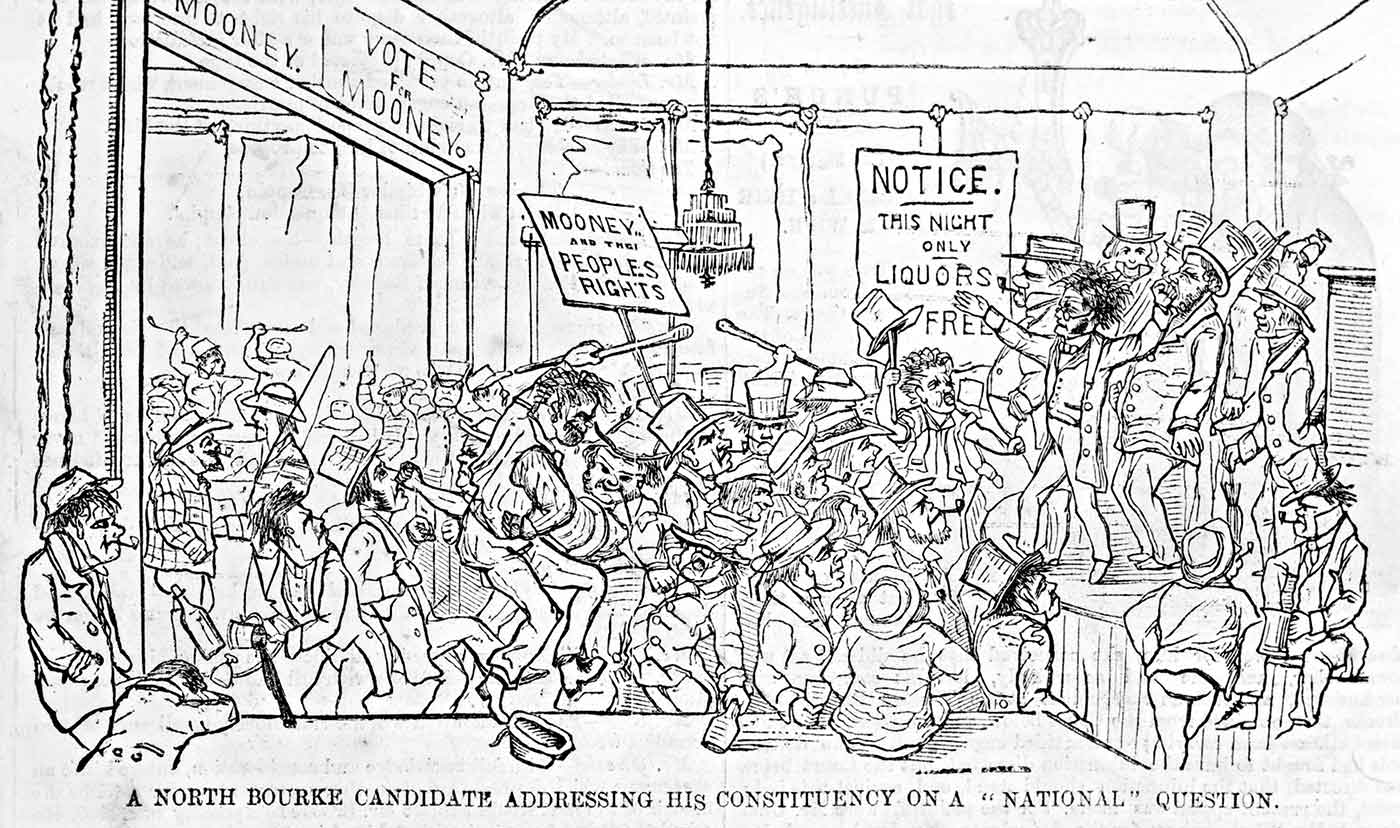
\includegraphics[scale=0.25]{NorthBourke.jpg}
	\caption{Election held in 1855 in Victoria, Australia 
	  was conducted in pub!}
	\end{center}
  \end{figure}   
  
